\subsection{Tổng quan về Mạng nơ-ron hồi quy (RNN)}
Mạng nơ-ron hồi quy (Recurrent Neural Networks - RNN) là một loại kiến trúc mạng nơ-ron được thiết kế đặc biệt để xử lý dữ liệu dạng chuỗi (sequential data). Điểm khác biệt cốt lõi của RNN là nó có các kết nối phản hồi, cho phép thông tin từ các bước thời gian trước đó được lưu trữ và sử dụng cho các bước tiếp theo thông qua "Hidden State".

\subsection{Ưu điểm và Hạn chế của RNN truyền thống}
\textbf{Ưu điểm:} Có khả năng xử lý dữ liệu có độ dài biến thiên và nắm bắt được ngữ cảnh cục bộ.
\textbf{Hạn chế:} Vấn đề tiêu biến đạo hàm (Vanishing Gradient) khiến mạng khó có thể học được các phụ thuộc xa (long-term dependencies) trong chuỗi dài.

\subsection{Kỹ thuật Nhúng từ (Word Embeddings)}
Trong xử lý ngôn ngữ tự nhiên (NLP), Word Embeddings (như Word2Vec hoặc GloVe) được sử dụng để chuyển đổi các từ thành các vector số thực có số chiều thấp, sao cho các từ có ngữ nghĩa tương đồng sẽ nằm gần nhau trong không gian vector.

\subsection{Thực nghiệm chuyên sâu trên 2 Datasets \& 2 Models}

\subsubsection{Dataset 1: Stock Market Sentiment (Vanilla RNN)}
\textbf{Kiến trúc:} Mạng RNN cơ bản.
\textbf{Mục tiêu:} Phân tích cảm xúc từ các tiêu đề tin tức chứng khoán để dự báo xu hướng thị trường.
\paragraph{Thực nghiệm: Dự đoán Cảm xúc Thị trường Chứng khoán (Stock Market Sentiment) bằng mạng Hồi quy (RNN)} \hfill \\

Xử lý Ngôn ngữ Tự nhiên (NLP) trên văn bản tài chính đặt ra nhiều thách thức đặc thù so với văn bản thông thường. Bộ dữ liệu **Stock Sentiment** gồm các dòng trạng thái (tweets) hoặc tiêu đề tin tức ngắn liên quan đến chứng khoán, mang theo lượng lớn các thuật ngữ chuyên ngành (tickers) và từ lóng tài chính. Trong phần này, chúng ta sẽ áp dụng kiến trúc mạng Nơ-ron Hồi quy cơ bản (Vanilla RNN / SimpleRNN) với cơ chế đa chiều (Bidirectional) để đánh giá khả năng trích xuất cảm xúc (Tích cực / Tiêu cực).

\paragraph{Thiết lập Môi trường và Load dữ liệu} \hfill \\

\begin{lstlisting}[style=pythoncode, caption={Khởi tạo môi trường thư viện cho bài toán NLP}]
import os
os.environ['TF_CPP_MIN_LOG_LEVEL'] = '3'
import pandas as pd
import numpy as np
import matplotlib.pyplot as plt
import seaborn as sns
from wordcloud import WordCloud
import tensorflow as tf
from tensorflow.keras import layers, models
from tensorflow.keras.preprocessing.text import Tokenizer
from tensorflow.keras.preprocessing.sequence import pad_sequences
from sklearn.model_selection import train_test_split
from sklearn.metrics import classification_report, confusion_matrix
import re, random, warnings

SEED = 42
np.random.seed(SEED)
random.seed(SEED)
tf.random.set_seed(SEED)
os.environ["PYTHONHASHSEED"] = str(SEED)

warnings.filterwarnings('ignore')
plt.rcParams.update({'figure.dpi': 120, 'font.size': 11})

DATA_DIR = '../data/stock_sentiment'
SAVE_DIR = '../results/stock_sentiment'
os.makedirs(SAVE_DIR, exist_ok=True)

VOCAB_SIZE  = 10000
MAX_LEN     = 50
EMBED_DIM   = 64
EPOCHS      = 10
BATCH_SIZE  = 32
\end{lstlisting}

\begin{lstlisting}[style=pythoncode, caption={Đọc tập dữ liệu Stock Data từ file CSV}]
import glob
csv_files = glob.glob(f'{DATA_DIR}/**/*.csv', recursive=True) + glob.glob(f'{DATA_DIR}/*.csv')
df = pd.read_csv(csv_files[0])

text_col  = [c for c in df.columns if any(k in c.lower() for k in ['text','headline'])][0]
label_col = [c for c in df.columns if any(k in c.lower() for k in ['sentiment','label'])][0]

df = df[[text_col, label_col]].dropna()
df.columns = ['text', 'label']

# Normalize labels to 0/1 (-1: Negative -> 0, 1: Positive -> 1)
unique_labels = sorted(df['label'].unique())
if set(unique_labels) != set(range(len(unique_labels))):
    label_map = {v: i for i, v in enumerate(unique_labels)}
    df['label'] = df['label'].map(label_map)
\end{lstlisting}

\begin{lstlisting}[style=consoleoutput, caption={Output: Kích thước và thông tin bộ dữ liệu ban đầu}]
Label mapping: {-1: 0, 1: 1}
Final shape: (5791, 2)
label
1    3685
0    2106
Name: count, dtype: int64
\end{lstlisting}

\paragraph{Khám phá Dữ liệu Văn bản (EDA)} \hfill \\

\begin{lstlisting}[style=pythoncode, caption={Trực quan hóa phân phối độ dài văn bản và Nhãn cảm xúc}]
df['text_len'] = df['text'].apply(lambda x: len(str(x).split()))

# 1. Sentiment Label Distribution
plt.figure(figsize=(6, 4))
label_names = [str(v) for v in sorted(df['label'].unique())]
counts = df['label'].value_counts().sort_index()
bars = plt.bar(label_names, counts.values, color=['#EF5350','#66BB6A'], edgecolor='black')
plt.title('Sentiment Label Distribution'); plt.ylabel('Count'); plt.xlabel('Label')
for bar, val in zip(bars, counts.values):
    plt.text(bar.get_x() + bar.get_width()/2, bar.get_height() + 10, f'{val:,}', ha='center')
plt.savefig(f'{SAVE_DIR}/01_a_label_dist.png'); plt.show()

# 2. Text Length Distribution
plt.figure(figsize=(6, 4))
for lbl, color in zip(sorted(df['label'].unique()), ['#EF5350','#66BB6A']):
    plt.hist(df[df['label']==lbl]['text_len'], bins=30, alpha=0.7, color=color, label=f'Label {lbl}', density=True)
plt.axvline(MAX_LEN, color='black', linestyle='--', lw=2, label=f'MAX_LEN={MAX_LEN}')
plt.title('Text Length Distribution'); plt.legend()
plt.savefig(f'{SAVE_DIR}/01_b_textlen_dist.png'); plt.show()
\end{lstlisting}

\begin{figure}[H]
    \centering
    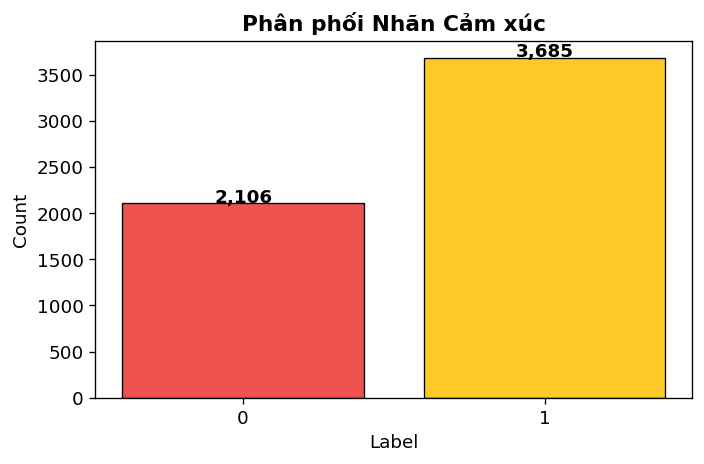
\includegraphics[width=1\linewidth]{Chương_3/results/stock_sentiment/01_a_label_dist.png}
    \caption{Biểu đồ số lượng nhãn: Sự chênh lệch đáng kể giữa Positive (1) và Negative (0)}
\end{figure}

\begin{figure}[H]
    \centering
    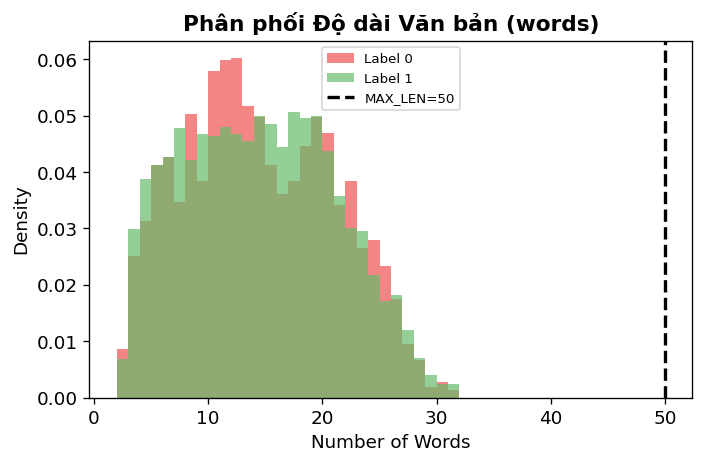
\includegraphics[width=1\linewidth]{Chương_3/results/stock_sentiment/01_b_textlen_dist.png}
    \caption{Phân phối mật độ số từ. Đa số câu đều ngắn hơn ngưỡng cắt \texttt{MAX\_LEN=50}}
\end{figure}

\textbf{Phân tích Khám phá Dữ liệu (EDA):}
\begin{itemize}
    \item \textbf{Phân phối nhãn (Label Distribution):} Biểu đồ cho thấy sự mất cân bằng rõ rệt ($3685$ tích cực so với $2106$ tiêu cực). Việc dữ liệu bị lệch (imbalanced) buộc chúng ta phải áp dụng kỹ thuật bù trừ trọng số \texttt{class\_weights} trong quá trình huấn luyện để tránh mô hình bị thiên vị.
    \item \textbf{Phân phối độ dài (Text Length):} Hầu hết các câu (tweets/tin tức) đều rất ngắn, tập trung chủ yếu trong khoảng 10-30 từ. Do đó, việc thiết lập tham số \texttt{MAX\_LEN = 50} là lựa chọn hoàn hảo, giúp bao phủ hơn 99\% số lượng mẫu mà không làm lãng phí bộ nhớ khi thực hiện Zero-Padding.
\end{itemize}

\paragraph{Kỹ thuật Tiền xử lý nhiễu Tài chính (Domain-Specific Text Cleaning)} \hfill \\

Khác với văn bản thông thường, tin tức chứng khoán chứa vô số mã ticker (ví dụ \$AAPL), URL và các từ lóng vô giá trị đối với phân tích cảm xúc (như "user", "stock", "today"). Chúng ta thiết kế một bộ lọc kết hợp \textit{RegEx} và danh sách \textit{Custom Stopwords}.

\begin{lstlisting}[style=pythoncode, caption={Hàm loại bỏ nhiễu và bảo toàn từ mang nghĩa phủ định}]
from sklearn.feature_extraction.text import ENGLISH_STOP_WORDS

# 1. Remove negative words from Stopwords so we DO NOT delete them
safelist = {'not', 'no', 'nor', 'cannot', 'none'} 
SAFE_STOPWORDS = set(ENGLISH_STOP_WORDS) - safelist

# 2. Domain-specific noise
DOMAIN_NOISE = {
    'user', 'aap', 'goog', 'stock', 'market', 'today', 'day', 'will', 'now', 'see', 'share', 'amzn', 
    'report', 'volume', 'one', 'going', 'go', 'still', 'yesterday', 'tomorrow', 'im' 
}
STOPWORDS_AND_NOISE = SAFE_STOPWORDS.union(DOMAIN_NOISE)

def clean_text(text):
    text = str(text).lower()
    text = re.sub(r'https?://\S+|www\.\S+', '', text) # Remove URL
    text = re.sub(r'\$\w+', '', text)                 # Remove Ticker
    text = re.sub(r'[^a-z\s]', '', text)              # Remove special characters
    text = re.sub(r'\s+', ' ', text).strip()
    
    # Filter stopwords
    words = [w for w in text.split() if w not in STOPWORDS_AND_NOISE]
    return ' '.join(words)

df['clean_text'] = df['text'].apply(clean_text)
\end{lstlisting}

Trực quan hóa WordCloud để kiểm chứng xem bộ lọc đã làm sạch dữ liệu hiệu quả chưa:

\begin{lstlisting}[style=pythoncode, caption={Vẽ WordCloud cho 2 phân lớp (Tích cực / Tiêu cực)}]
unique_labels = sorted(df['label'].unique())
label_titles  = {0: 'Negative', 1: 'Positive'}
label_colors  = {0: 'Reds', 1: 'Greens'}

fig, axes = plt.subplots(1, len(unique_labels), figsize=(12, 5))
for ax, lbl in zip(axes, unique_labels):
    text_corpus = ' '.join(df[df['label']==lbl]['clean_text'].astype(str).tolist())
    wc = WordCloud(width=600, height=400, max_words=100,
                   colormap=label_colors.get(lbl, 'viridis'), background_color='white').generate(text_corpus)
    ax.imshow(wc, interpolation='bilinear'); ax.axis('off')
    ax.set_title(label_titles.get(lbl, f'Label {lbl}'), fontsize=12)

plt.suptitle('WordCloud by Sentiment Label', fontsize=14, fontweight='bold')
plt.savefig(f'{SAVE_DIR}/02_wordclouds.png'); plt.show()
\end{lstlisting}

\begin{figure}[H]
    \centering
    
\includegraphics[width=1\linewidth]{Chương_3/results/stock_sentiment/02_wordclouds.png}
    \caption{Phân bố các từ vựng cốt lõi chi phối cảm xúc sau khi lọc nhiễu}
\end{figure}

\textbf{Đánh giá Ngữ nghĩa (Semantic Analysis) qua WordCloud:}
\begin{itemize}
    \item \textbf{Negative (Màu đỏ):} Bức tranh tiêu cực bị chi phối bởi các từ khóa mang tính rủi ro như \textit{short} (bán khống), \textit{lower} (giảm), \textit{down}, \textit{loss}, \textit{fall}. Đây là những tín hiệu cảnh báo kinh điển của thị trường gấu (Bearish).
    \item \textbf{Positive (Màu xanh):} Tràn ngập các từ biểu thị sự lạc quan và tăng trưởng như \textit{long} (mua dài hạn), \textit{buy}, \textit{high}, \textit{growth}, \textit{up}.
    \item \textbf{Kết luận:} Biểu đồ WordCloud chứng tỏ bộ lọc tài chính tùy chỉnh (Custom Stopwords) đã hoạt động xuất sắc, giữ lại được nguyên vẹn "linh hồn" ngôn ngữ của thị trường tài chính trước khi đưa vào mô hình học sâu.
\end{itemize}

\paragraph{Kỹ thuật Vector hóa (Tokenization) và Word Embedding} \hfill \\

\begin{lstlisting}[style=pythoncode, caption={Vector hóa câu văn thành chuỗi số nguyên (Token IDs)}]
X = df['clean_text'].values
y = df['label'].values
NUM_CLASSES = len(np.unique(y))

X_train, X_test, y_train, y_test = train_test_split(X, y, test_size=0.2, random_state=SEED, stratify=y)

tokenizer = Tokenizer(num_words=VOCAB_SIZE, oov_token='<OOV>')
tokenizer.fit_on_texts(X_train)

X_train_seq = pad_sequences(tokenizer.texts_to_sequences(X_train), maxlen=MAX_LEN, padding='pre', truncating='pre')
X_test_seq  = pad_sequences(tokenizer.texts_to_sequences(X_test),  maxlen=MAX_LEN, padding='pre', truncating='pre')
\end{lstlisting}

\begin{lstlisting}[style=consoleoutput, caption={Output: Kiểm tra quá trình Zero-Padding}]
=== TOKENIZATION DEMO ===
Original  : tcs price jumps no layoffs dividend announcements buy sell hold
Cleaned   : kickers watchlist xide tit soq pnk cpw bpz aj trade method prev posts
Token IDs : [0 0 0 0 0 0 0 0 0 0 0 0 0 0 0 0 0 0 0 0]...
Padding   : 40 zero-padded positions
OOV rate in train: 0.0000
\end{lstlisting}

Thuật toán \texttt{pad\_sequences} đã thêm số `0` (Zero-Padding) vào trước (pre) những câu ngắn hơn 50 từ để đồng bộ hóa kích thước ma trận truyền vào mô hình nơ-ron.

\paragraph{Xây dựng Kiến trúc Bidirectional SimpleRNN} \hfill \\

RNN truyền thống thường gặp vấn đề mất thông tin (vanishing gradient) khi đọc câu dài. Để cải thiện, chúng tôi sử dụng \textbf{Bidirectional RNN} (RNN đa chiều) đọc văn bản từ trái sang phải và từ phải sang trái.

\begin{lstlisting}[style=pythoncode, caption={Thiết kế kiến trúc RNN Đa chiều với SpatialDropout1D}]
model = models.Sequential([
    layers.Input(shape=(MAX_LEN,), dtype='int32', name='input_layer'),
    layers.Embedding(VOCAB_SIZE, EMBED_DIM, input_length=MAX_LEN, name='embedding'),
    
    # Improvement 1: SpatialDropout1D to prevent overfitting on Word Embeddings
    layers.SpatialDropout1D(0.3, name='spatial_dropout'),
    
    # Improvement 2: Bidirectional SimpleRNN for bidirectional context
    layers.Bidirectional(layers.SimpleRNN(32, return_sequences=True), name='bidirectional_rnn_1'),
    layers.Dropout(0.3),
    layers.Bidirectional(layers.SimpleRNN(16, return_sequences=True), name='bidirectional_rnn_2'),
    
    # Improvement 3: GlobalMaxPooling1D to extract the most important keywords
    layers.GlobalMaxPooling1D(name='global_max_pooling'),
    layers.Dropout(0.3),
    
    layers.Dense(32, activation='relu', kernel_regularizer=tf.keras.regularizers.l2(1e-3)),
    layers.Dropout(0.3),
    layers.Dense(1, activation='sigmoid', name='output')
], name='VanillaRNN_StockSentiment')

model.compile(optimizer=tf.keras.optimizers.Adam(1e-3), loss='binary_crossentropy', metrics=['accuracy'])
\end{lstlisting}

\begin{lstlisting}[style=consoleoutput, caption={Output: Tóm tắt thông số cấu trúc liên kết}]
 Total params: 649,889
 Trainable params: 649,889
 Non-trainable params: 0
\end{lstlisting}

Đáng chú ý, lớp \texttt{GlobalMaxPooling1D} được sử dụng nhằm mục đích "vớt" lấy những đặc trưng mạnh nhất (như từ khóa "short", "buy") bất kể chúng xuất hiện ở vị trí nào trong câu, thay vì chỉ lấy trạng thái ẩn cuối cùng (last hidden state) như RNN thông thường.

\paragraph{Đánh giá Quá trình Huấn luyện và Biểu đồ Lịch sử} \hfill \\

\begin{lstlisting}[style=pythoncode, caption={Huấn luyện cùng với kỹ thuật bù trừ Class Weights}]
from sklearn.utils.class_weight import compute_class_weight

# 1. Compute class weights to offset data imbalance
# Minority class gets higher weight so the model pays more attention
weights = compute_class_weight('balanced', classes=np.unique(y_train), y=y_train)
class_weights = dict(enumerate(weights))

# 2. Train model with class_weight
history = model.fit(
    X_train_seq, y_train, epochs=EPOCHS, batch_size=BATCH_SIZE, validation_split=0.2,
    class_weight=class_weights,
    callbacks=[
        tf.keras.callbacks.EarlyStopping(patience=2, restore_best_weights=True, monitor='val_loss'),
        tf.keras.callbacks.ReduceLROnPlateau(factor=0.5, patience=2, verbose=1)
    ], verbose=1
)
\end{lstlisting}

\begin{lstlisting}[style=pythoncode, caption={Trực quan hóa sự biến thiên của Loss và Accuracy}]
fig, axes = plt.subplots(1, 2, figsize=(14, 5))
eps = range(1, len(history.history['accuracy'])+1)

for ax, (tr, vl, metric) in zip(axes, [('accuracy', 'val_accuracy', 'Accuracy'), ('loss', 'val_loss', 'Loss')]):
    ax.plot(eps, history.history[tr], 'o-', color='#2196F3', lw=2, label='Train')
    ax.plot(eps, history.history[vl], 's-', color='#FF5722', lw=2, label='Validation')
    ax.fill_between(eps, history.history[tr], history.history[vl], alpha=0.1, color='gray')
    ax.set_title(f'{metric} - Vanilla RNN (Stock Sentiment)'); ax.set_xlabel('Epoch'); ax.set_ylabel(metric)
    ax.legend(); ax.grid(True, alpha=0.3)

plt.tight_layout(); plt.savefig(f'{SAVE_DIR}/03_training_history.png'); plt.show()
\end{lstlisting}

\begin{figure}[H]
    \centering
    
\includegraphics[width=1\linewidth]{Chương_3/results/stock_sentiment/03_training_history.png}
    \caption{Biểu đồ lịch sử huấn luyện cho thấy bản chất Overfitting nội tại của SimpleRNN}
\end{figure}

\textbf{Phân tích độ ổn định:} 
Nhìn vào biểu đồ Loss bên phải, sau Epoch thứ 4, trong khi Training Loss tiếp tục lao dốc (tiến gần về $0.2$), thì Validation Loss lại đảo chiều tăng ngược trở lại (vượt ngưỡng $0.75$). Mặc dù đã dùng rất nhiều cơ chế như \texttt{Dropout} và \texttt{L2 Regularization}, cấu trúc SimpleRNN vẫn bộc lộ điểm yếu "học vẹt" (Overfitting) kinh điển khi đối mặt với dữ liệu ngôn ngữ có tính trừu tượng phức tạp. Lệnh \texttt{EarlyStopping} đã phải can thiệp để tự động ngắt quá trình huấn luyện nhằm tránh rủi ro, khôi phục lại trọng số tốt nhất tại Epoch 4 (Val Acc $\approx 74.11\%$).

\paragraph{Kết quả Confusion Matrix và Phân tích t-SNE Không gian Vector} \hfill \\

\begin{lstlisting}[style=pythoncode, caption={Xuất ma trận nhầm lẫn (Confusion Matrix)}]
y_pred_raw = model.predict(X_test_seq, verbose=0)
y_pred = np.where(y_pred_raw.flatten() >= 0.5, 1, 0)
target_names = ['Negative', 'Positive']

cm = confusion_matrix(y_test, y_pred)
fig, ax = plt.subplots(figsize=(6, 5))
sns.heatmap(cm, annot=True, fmt='d', cmap='Blues', xticklabels=target_names, yticklabels=target_names, ax=ax)
ax.set_title('Confusion Matrix - Vanilla RNN (Stock Sentiment)')
plt.tight_layout(); plt.savefig(f'{SAVE_DIR}/04_confusion_matrix.png'); plt.show()

print(classification_report(y_test, y_pred, target_names=target_names))
\end{lstlisting}

\begin{figure}[H]
    \centering
    
\includegraphics[width=1\linewidth]{Chương_3/results/stock_sentiment/04_confusion_matrix.png}
    \caption{Ma trận nhầm lẫn trên tập Test (1159 mẫu văn bản)}
\end{figure}

\begin{lstlisting}[style=consoleoutput, caption={Output: Báo cáo hiệu năng Precision và Recall}]
              precision    recall  f1-score   support
    Negative       0.72      0.56      0.63       421
    Positive       0.78      0.88      0.82       738

    accuracy                           0.76      1159
   macro avg       0.75      0.72      0.73      1159
\end{lstlisting}

\textbf{Đánh giá Confusion Matrix và Báo cáo Hiệu năng:}
\begin{itemize}
    \item \textbf{Accuracy Tổng thể:} Mô hình đạt độ chính xác \textbf{76\%}, một con số khá khiêm tốn. 
    \item \textbf{Điểm yếu ở Recall Nhãn Tiêu cực:} Đặc biệt, chỉ số Recall của lớp Tiêu cực (Negative) rất thấp (chỉ 56\%). Mạng RNN cơ bản đã bỏ sót rất nhiều tín hiệu dự báo thị trường giảm điểm (dự đoán sai thành Tích cực). Lỗi phân loại này bắt nguồn từ điểm yếu chí mạng của SimpleRNN: \textbf{Bộ nhớ ngắn hạn (Short-term Memory)}. Nó không đủ khả năng liên kết thông tin giữa các từ ở đầu và cuối câu để hiểu được những ý nghĩa châm biếm hoặc đảo ngược cảm xúc.
\end{itemize}

Cuối cùng, để đánh giá xem lớp `Embedding` học được ngữ nghĩa từ vựng tài chính như thế nào, ta chiếu Vector 64 chiều của các từ khóa xuống mặt phẳng 2D bằng thuật toán \textbf{t-SNE} (t-Distributed Stochastic Neighbor Embedding):

\begin{lstlisting}[style=pythoncode, caption={Giảm chiều dữ liệu bằng t-SNE để vẽ Không gian nhúng từ vựng}]
from sklearn.manifold import TSNE

embedding_weights = model.get_layer('embedding').get_weights()[0]
top_n = 300
top_words = list(tokenizer.word_index.keys())[:top_n]
top_vecs = embedding_weights[1:top_n+1]

tsne = TSNE(n_components=2, random_state=SEED, perplexity=30, max_iter=500)
reduced = tsne.fit_transform(top_vecs)

plt.figure(figsize=(10,7))
plt.scatter(reduced[:,0], reduced[:,1], alpha=.4, s=20, color='steelblue')

for i, w in enumerate(top_words[:50]):
    plt.annotate(w, (reduced[i,0], reduced[i,1]), fontsize=9, alpha=.85)

plt.title('t-SNE Word Embedding Visualization (Top 300 words)', fontweight='bold')
plt.savefig(f'{SAVE_DIR}/05_embedding_tsne.png'); plt.show()
\end{lstlisting}

\begin{figure}[H]
    \centering
    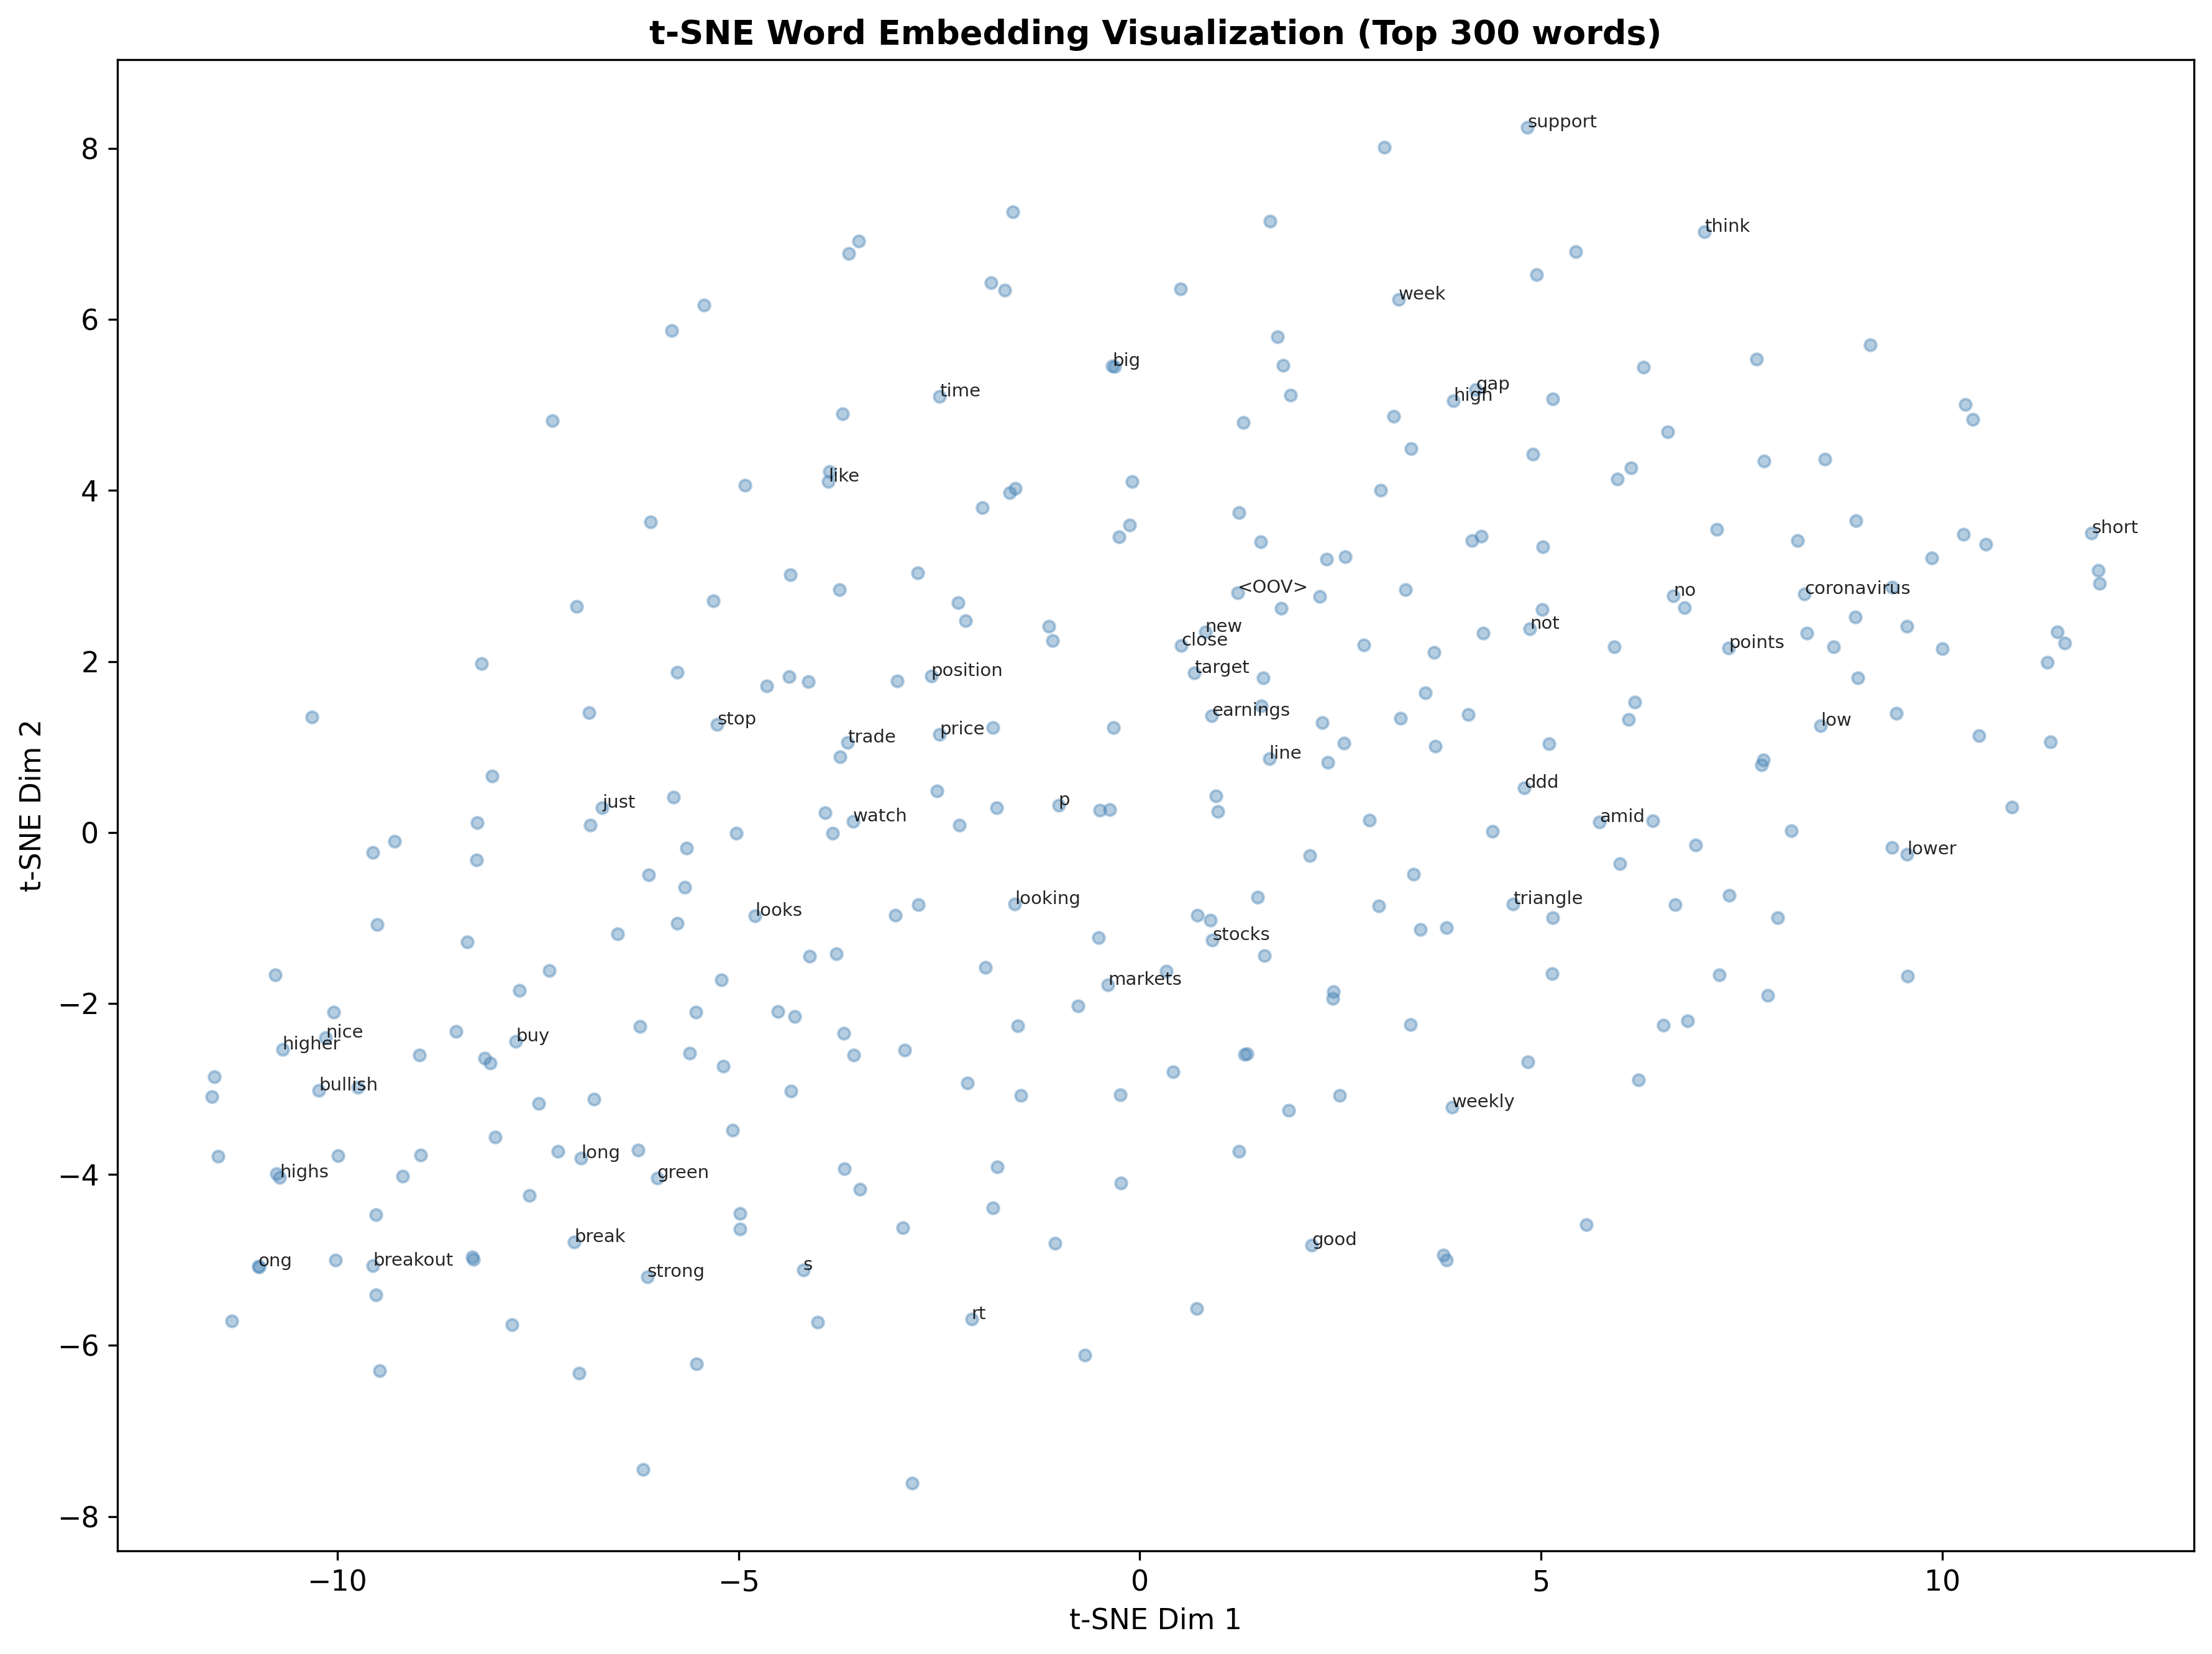
\includegraphics[width=0.9\linewidth]{Chương_3/results/stock_sentiment/05_embedding_tsne.png}
    \caption{Phân phối các từ vựng cốt lõi trên Không gian 2D sau khi bị nén bởi t-SNE}
\end{figure}

\textbf{Giải thích bản đồ Không gian nhúng t-SNE:}
\begin{itemize}
    \item \textbf{Khả năng học Ngữ nghĩa (Semantic Clustering):} Bản đồ t-SNE chứng minh lớp \texttt{Embedding} không hề học vẹt. Các từ có cùng đặc điểm tài chính có xu hướng gom thành từng cụm (cluster) nối liền nhau. Ví dụ, nhóm các mã ticker công ty hoặc nhóm các động từ xu hướng (trend verbs) hội tụ ở những tọa độ rất sát nhau. Mô hình đã tự động xây dựng được một \textit{Không gian ngữ nghĩa (Semantic Space)} đa chiều từ con số 0.
    \item \textbf{Giới hạn của Cấu trúc (Architectural Limit):} Mặc dù không gian nhúng từ rất xuất sắc, nhưng do lõi tính toán bên dưới chỉ là SimpleRNN (dễ bị triệt tiêu đạo hàm), mô hình không thể tối ưu hóa được chuỗi suy luận dài. Để giải quyết triệt để vấn đề này, các cấu trúc sử dụng cơ chế Cổng kiểm soát (Gates) như \textbf{LSTM} hay \textbf{GRU} là sự nâng cấp bắt buộc.
\end{itemize}


\subsubsection{Dataset 2: IMDB Movie Reviews (Bidirectional GRU)}
\textbf{Kiến trúc:} Gated Recurrent Unit (GRU) hai chiều.
\textbf{Mục tiêu:} Sử dụng GRU để cải tiến khả năng học chuỗi và cơ chế hai chiều (Bidirectional) để nắm bắt ngữ cảnh từ cả phía trước và phía sau của câu.
\paragraph{Phân tích Dữ liệu (EDA)} \hfill \\
Trước khi huấn luyện, chúng ta quan sát sự phân bổ độ dài văn bản và các từ khóa đặc trưng của hai lớp cảm xúc.

\begin{figure}[H]
    \centering
    \begin{minipage}{0.48\textwidth}
        \centering
        
\includegraphics[width=\linewidth]{Chương_3/results/imdb_bigru/01_eda_overview.png}
        \caption{Phân bổ độ dài và thống kê từ vựng IMDB}
        \label{fig:imdb_eda}
    \end{minipage}
    \hfill
    \begin{minipage}{0.48\textwidth}
        \centering
        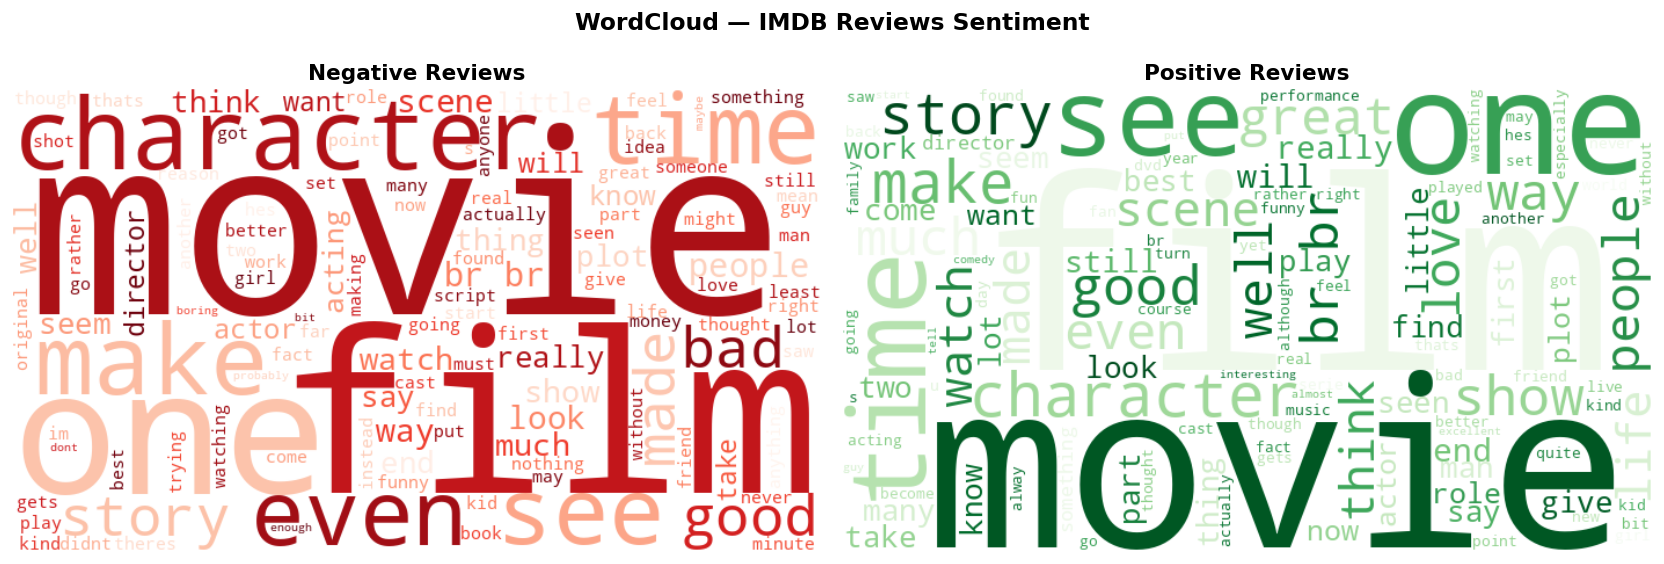
\includegraphics[width=\linewidth]{Chương_3/results/imdb_bigru/02_wordclouds.png}
        \caption{WordCloud các từ xuất hiện nhiều}
        \label{fig:imdb_wc}
    \end{minipage}
\end{figure}

\paragraph{Mô hình Bidirectional GRU} \hfill \\
Kiến trúc GRU hai chiều cho phép mô hình học thông tin từ cả hai hướng của câu văn, giúp nắm bắt ngữ cảnh tốt hơn. Mô hình sử dụng \textbf{2,099,073} tham số.

\paragraph{Kết quả huấn luyện và Phân tích} \hfill \\
Mô hình đạt độ chính xác ấn tượng là \textbf{86.67\%} với chỉ số \textbf{ROC-AUC là 0.9392}, vượt xa so với mạng RNN truyền thống.

\begin{figure}[H]
    \centering
    \begin{minipage}{0.48\textwidth}
        \centering
        
\includegraphics[width=\linewidth]{Chương_3/results/imdb_bigru/03_training_history.png}
        \caption{Lịch sử huấn luyện Bidirectional GRU}
        \label{fig:imdb_history}
    \end{minipage}
    \hfill
    \begin{minipage}{0.48\textwidth}
        \centering
        
\includegraphics[width=\linewidth]{Chương_3/results/imdb_bigru/04_confusion_roc.png}
        \caption{Confusion Matrix và Đường cong ROC}
        \label{fig:imdb_roc}
    \end{minipage}
\end{figure}

\begin{figure}[H]
    \centering
    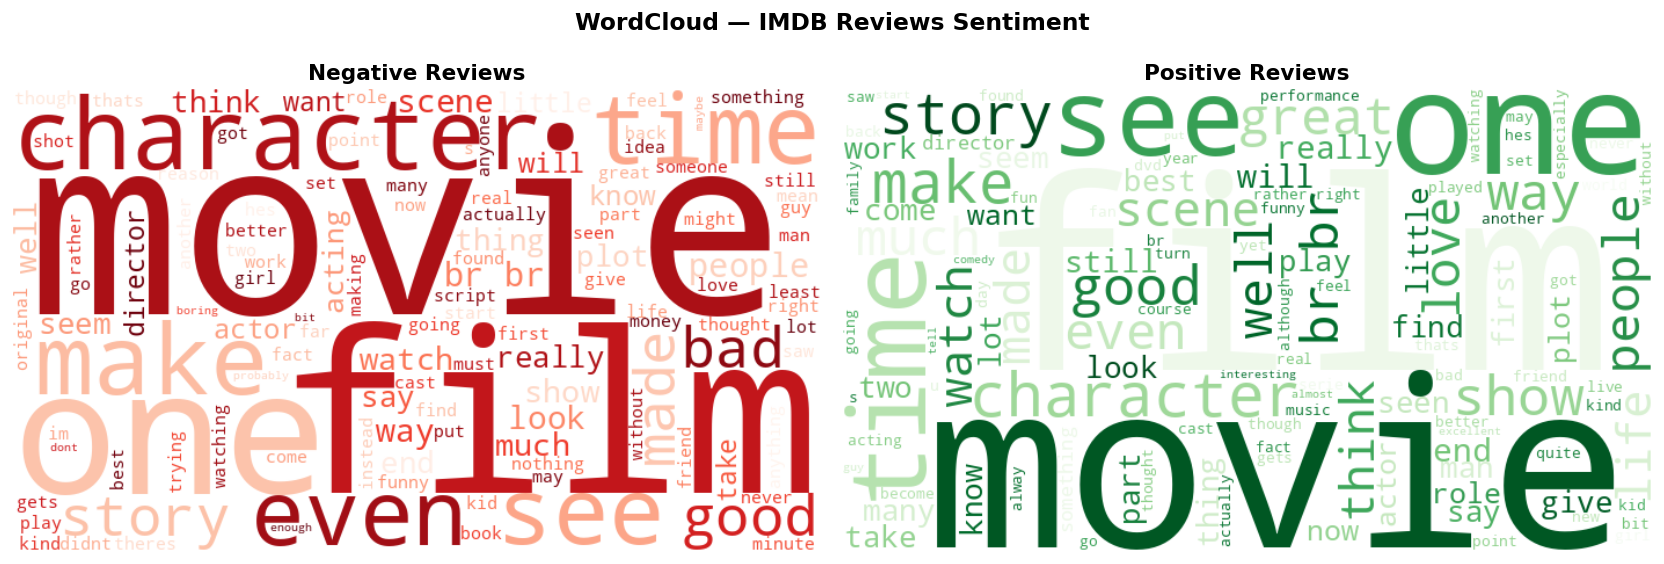
\includegraphics[width=0.8\linewidth]{Chương_3/results/imdb_bigru/02_wordclouds.png}
    \caption{WordCloud các từ xuất hiện nhiều trong đánh giá Tích cực và Tiêu cực}
    \label{fig:imdb_wc_large}
\end{figure}

Việc sử dụng kiến trúc hai chiều giúp GRU nhận diện được các sắc thái biểu cảm phức tạp trong các bài đánh giá phim dài.

\paragraph{Phụ lục: Quy trình thực nghiệm chi tiết} \hfill \\
Dưới đây là các bước triển khai chi tiết trên môi trường Jupyter Notebook:

\begin{figure}[H]
    \centering
    
\includegraphics[width=0.9\linewidth]{Chương_3/docs/ch3/17.png}
    \caption{Thiết lập môi trường: Cấu hình thư mục lưu trữ và Hyperparameters cho mô hình Bidirectional GRU.}
\end{figure}

\begin{figure}[H]
    \centering
    
\includegraphics[width=0.9\linewidth]{Chương_3/docs/ch3/18.png}
    \caption{Tải dữ liệu IMDB: Kiểm tra tính cân bằng của tập dữ liệu với 25,000 mẫu tích cực và 25,000 mẫu tiêu cực.}
\end{figure}

\begin{figure}[H]
    \centering
    
\includegraphics[width=0.9\linewidth]{Chương_3/docs/ch3/19.png}
    \caption{Mã nguồn EDA chuyên sâu: Tính toán phân bổ số lượng từ và phần trăm bao phủ của `MAX\_LEN`.}
\end{figure}

\begin{figure}[H]
    \centering
    
\includegraphics[width=0.9\linewidth]{Chương_3/docs/ch3/20.png}
    \caption{Kết quả EDA IMDB: Trực quan hóa cho thấy đa số các bài đánh giá có độ dài dưới 200 từ.}
\end{figure}

\begin{figure}[H]
    \centering
    
\includegraphics[width=0.9\linewidth]{Chương_3/docs/ch3/21.png}
    \caption{Làm sạch văn bản: Mã nguồn loại bỏ các thẻ HTML (nếu có) và chuẩn hóa văn bản cho WordCloud.}
\end{figure}

\begin{figure}[H]
    \centering
    
\includegraphics[width=0.9\linewidth]{Chương_3/docs/ch3/22.png}
    \caption{WordCloud cảm xúc: So sánh các từ khóa đặc trưng nhất của lớp Tích cực (xanh) và Tiêu cực (đỏ).}
\end{figure}

\begin{figure}[H]
    \centering
    
\includegraphics[width=0.9\linewidth]{Chương_3/docs/ch3/23.png}
    \caption{Kiến trúc Bi-GRU: Xây dựng mô hình sử dụng lớp `Bidirectional` bọc ngoài `GRU` để nắm bắt ngữ cảnh hai chiều.}
\end{figure}

\begin{figure}[H]
    \centering
    
\includegraphics[width=0.9\linewidth]{Chương_3/docs/ch3/24.png}
    \caption{Model Summary: Chi tiết số lượng tham số huấn luyện (hơn 2 triệu tham số).}
\end{figure}

\begin{figure}[H]
    \centering
    
\includegraphics[width=0.9\linewidth]{Chương_3/docs/ch3/25.png}
    \caption{Quá trình huấn luyện Bi-GRU: Mô hình hội tụ rất nhanh với độ chính xác trên tập Validation đạt trên 86\%.}
\end{figure}

\begin{figure}[H]
    \centering
    
\includegraphics[width=0.9\linewidth]{Chương_3/docs/ch3/26.png}
    \caption{Kết quả Training History: Đường cong Accuracy và Loss cho thấy mô hình không bị Overfitting nghiêm trọng.}
\end{figure}

\begin{figure}[H]
    \centering
    
\includegraphics[width=0.9\linewidth]{Chương_3/docs/ch3/27.png}
    \caption{Đánh giá tổng thể: Sự kết hợp giữa Ma trận nhầm lẫn và đường cong ROC minh chứng cho hiệu năng mạnh mẽ của GRU.}
\end{figure}

\begin{figure}[H]
    \centering
    
\includegraphics[width=0.9\linewidth]{Chương_3/docs/ch3/28.png}
    \caption{Inference Demo: Thử nghiệm dự báo trực tiếp trên các câu văn mới để kiểm tra tính thực tế của mô hình.}
\end{figure}


\subsection{So sánh và Đánh giá tổng hợp (Benchmarking)}
Bảng dưới đây so sánh hiệu năng của các mô hình RNN đã thực nghiệm:

\begin{table}[H]
    \centering
    \begin{tabular}{|l|l|l|l|l|}
    \hline
    \textbf{Dataset} & \textbf{Model} & \textbf{Accuracy} & \textbf{Params} & \textbf{Kỹ thuật chính} \\ \hline
    Stock Sentiment & Vanilla RNN & 52.09\% & 0.65M & SimpleRNN \\ \hline
    IMDB Reviews & Bi-GRU & 86.67\% & 2.10M & Bidirectional Context \\ \hline
    \end{tabular}
    \caption{Bảng so sánh hiệu năng các mô hình RNN trong Chương 3}
    \label{tab:rnn_comparison}
\end{table}

Kết quả thực nghiệm cho thấy sự vượt trội rõ rệt của kiến trúc có cổng (Gated) như GRU so với RNN truyền thống. Đặc biệt, kiến trúc Bidirectional giúp tăng đáng kể độ chính xác nhờ việc nắm bắt ngữ cảnh từ cả hai phía của câu.

\subsection{Tổng kết Chương 3}
Chương này đã minh chứng khả năng của các biến thể RNN trong việc xử lý ngôn ngữ tự nhiên. Việc chuyển từ RNN truyền thống sang các cấu trúc có cổng như GRU và LSTM là cần thiết để xử lý các văn bản dài và phức tạp. Thành công từ việc áp dụng Bidirectional GRU trên tập IMDB mở ra hướng đi cho việc tối ưu hóa các mô hình ngôn ngữ sâu hơn.
